\documentclass[12pt]{article}

\usepackage[letterpaper, hmargin=0.75in, vmargin=0.75in]{geometry}
\usepackage{float}
\usepackage{graphicx}

% Fill in these values to make your life easier
\newcommand{\iterations}{???}
\newcommand{\physicalcores}{?}
\newcommand{\virtualcpus}{?}

\pagestyle{empty}

\title{Programming for Performance\\Assignment 1}
\author{Your Name}
\date{January 30, 2013}

\begin{document}

\maketitle

\section*{Part 2 - Benchmarking}

These experiments were run on a ??? CPU. It has \physicalcores{} physical cores and \virtualcpus{} virtual
CPUs.

\begin{table}[H]
  \centering
  \begin{tabular}{lr}
    & {\bf Time (s)} \\
    \hline
    Run 1 & 0 \\
    Run 2 & 0 \\
    Run 3 & 0 \\
    Run 4 & 0 \\
    Run 5 & 0 \\
    Run 6 & 0 \\
    \hline
    Average & 0 \\
  \end{tabular}
  \caption{Benchmark results for sequential execution ({\tt i} = \iterations{})}
  \label{tbl_sequential}
\end{table}

Refer to {\bf Table~\ref{tbl_sequential}} and estimate runtime with
\physicalcores{} physical cores.

\begin{table}[H]
  \centering
  \begin{tabular}{lr}
    & {\bf Time (s)} \\
    \hline
    Run 1 & 0 \\
    Run 2 & 0 \\
    Run 3 & 0 \\
    Run 4 & 0 \\
    Run 5 & 0 \\
    Run 6 & 0 \\
    \hline
    Average & 0 \\
  \end{tabular}
  \caption{Benchmark results for parallel execution ({\tt i} = \iterations{},
    {\tt t} = \physicalcores{})}
  \label{tbl_parallel_physicalcores}
\end{table}

Refer to {\bf Table~\ref{tbl_parallel_physicalcores}}, does this agree with your
predicted runtime? Write your answer here.

\begin{table}[H]
  \centering
  \begin{tabular}{lr}
    & {\bf Time (s)} \\
    \hline
    Run 1 & 0 \\
    Run 2 & 0 \\
    Run 3 & 0 \\
    Run 4 & 0 \\
    Run 5 & 0 \\
    Run 6 & 0 \\
    \hline
    Average & 0 \\
  \end{tabular}
  \caption{Benchmark results for parallel execution ({\tt i} = \iterations{},
    {\tt t} = \virtualcpus{})}
  \label{tbl_parallel_virtualcpus}
\end{table}

Refer to {\bf Table~\ref{tbl_parallel_virtualcpus}} calculate the speedup, and
verify it is less than \virtualcpus{}.

\begin{table}[H]
  \centering
  \begin{tabular}{lr}
    & {\bf Time (s)} \\
    \hline
    Run 1 & 0 \\
    Run 2 & 0 \\
    Run 3 & 0 \\
    Run 4 & 0 \\
    Run 5 & 0 \\
    Run 6 & 0 \\
    \hline
    Average & 0 \\
  \end{tabular}
  \caption{Benchmark results for parallel execution ({\tt i} = \iterations{},
    {\tt t} = \virtualcpus{} + 1)}
  \label{tbl_parallel_virtualcpus_plus_one}
\end{table}

Refer to {\bf Table~\ref{tbl_parallel_virtualcpus_plus_one}}, calculate the
speedup and compare it to {\bf Table~\ref{tbl_parallel_virtualcpus}} (or
{\bf Table~\ref{tbl_parallel_physicalcores}} if you don't have hyperthreading),
which performs better? Write your explanation here.


\begin{figure}[!ht]
	\centering
%  \includegraphics[height = 0.5\linewidth, width=0.7\linewidth]{24Templates.eps}
%	 \includegraphics[height = 0.3\linewidth, width=0.5\linewidth]{24Templates.eps} 
	 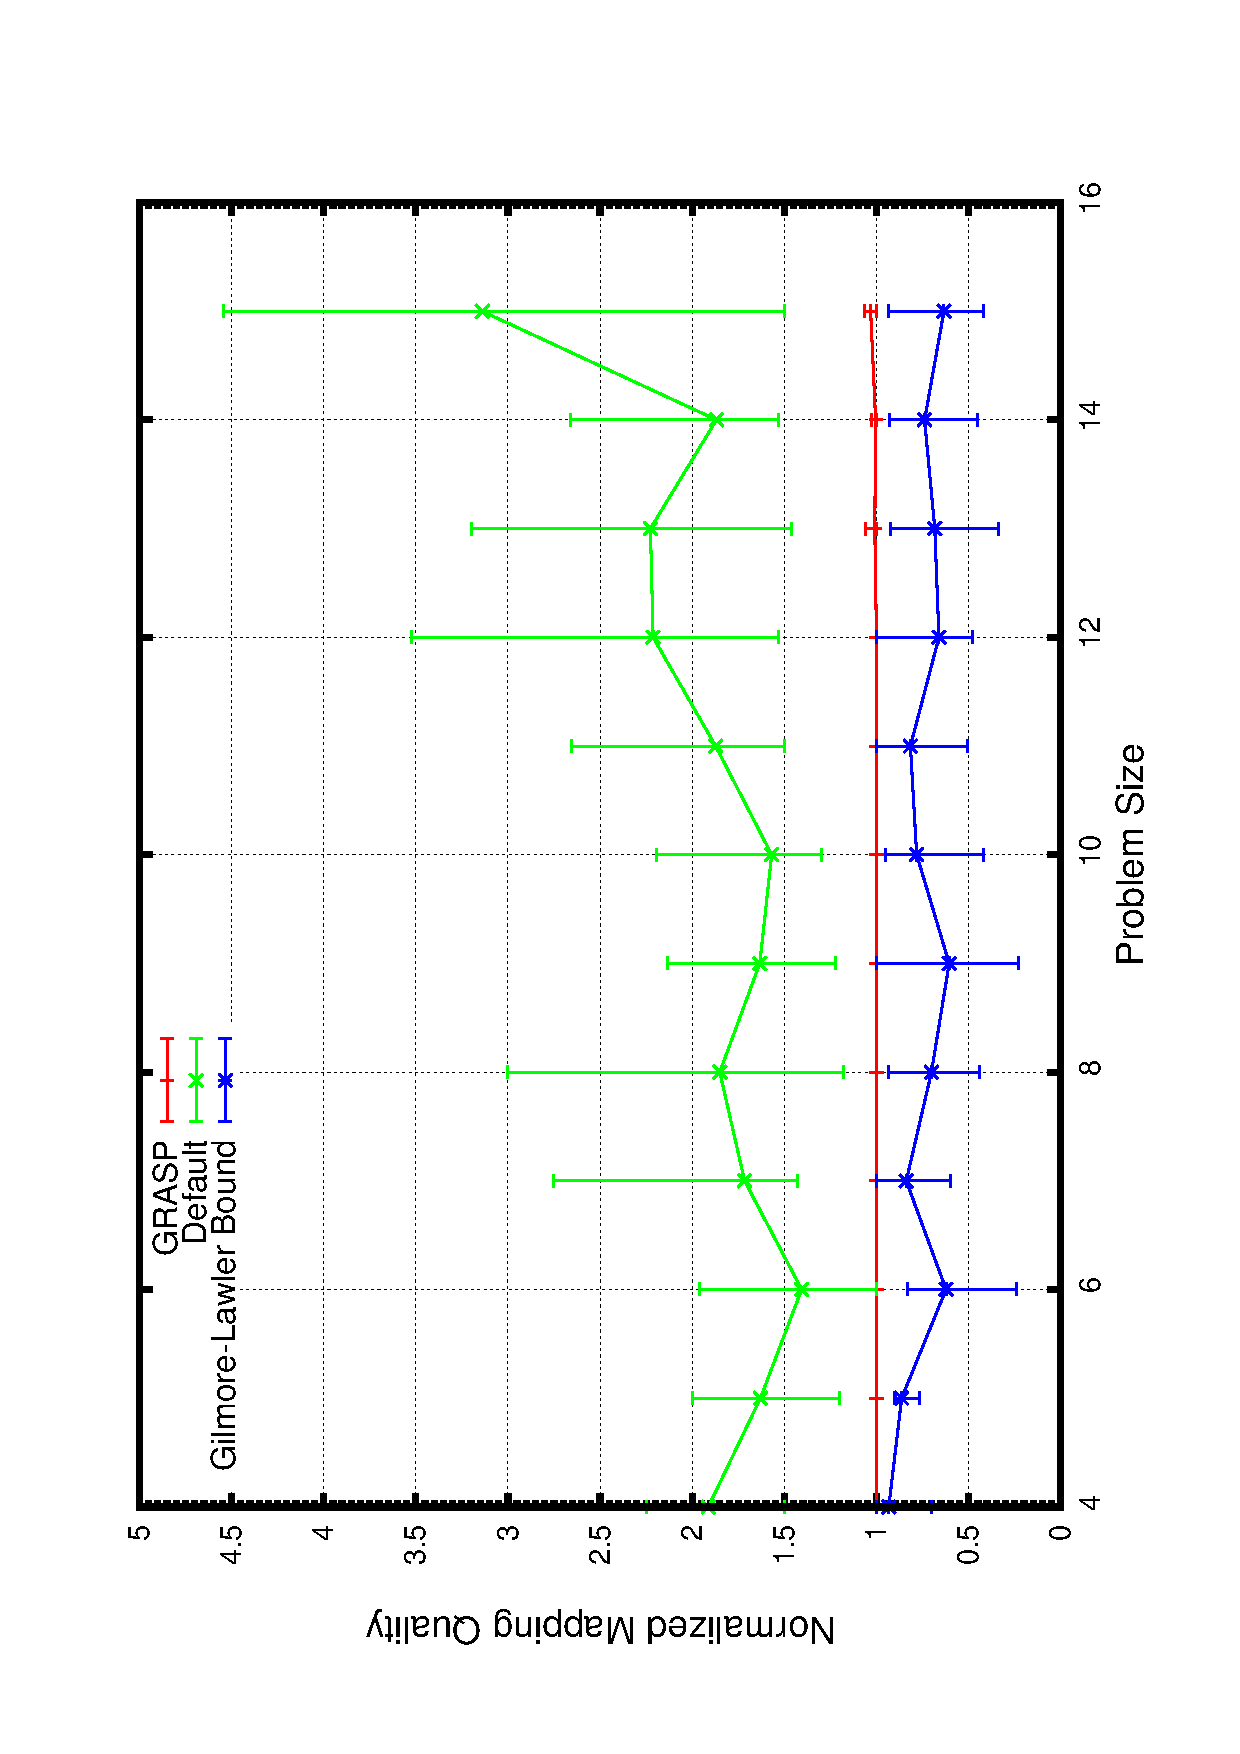
\includegraphics[width=0.7\linewidth, angle=270]{binomialfinalexactA} 
  \caption{Quality of solutions on the binomial tree pattern for small problem sizes.}
  \label{fig:bt-small}
\end{figure}
%

\begin{table}[ht]
\caption{Hops per Byte} % title of Table
\centering % used for centering table
\begin{tabular}{c c c c c c} % centered columns (4 columns)
\hline %inserts double horizontal lines
ProblemSize & GRASP & EMAHD & Default & GGE & MAHD\\  % inserts table
%heading
\hline % inserts single horizontal line
%1 & 50 & 837 & 970 \\ % inserting body of the table
8	& 1.43	& 1.48	& 2.22	& 2.18	& 1.83\\
16	& 2.98 &	3.76 &	5.36	& 3.88	& 4.02\\ 
32	& 2.94	& 4.05	& 5.88	& 5.19	& 4.30 \\ 
64	& 4.34	& 4.72	& 8.19	& 6.04	& 5.43 \\
100	& 2.56	& 2.74	& 3.84	& 3.86	& 3.16 \\
128	& 2.92	& 2.91	& 3.49	& 4.21	& 3.51 \\
144	& 2.73	& 2.61	& 4.25	& 4.16	& 3.22 \\
192	& 3.73	& 3.56	& 5.12	& 5.37	& 4.06 \\
200	& 3.14	& 2.77	& 4.30	& 4.05	& 2.83 \\
216	& 1.84	& 1.73	& 2.99	& 2.83	& 1.90 \\
250	& 3.66	& 3.39	& 5.50	& 5.37	& 3.45 \\
300	& 3.42	& 3.29	& 5.66	& 5.16	& 3.73 \\ [1ex] % [1ex] adds vertical space
\hline %inserts single line
\end{tabular}
\label{table:nonlin} % is used to refer this table in the text
\end{table}

\end{document}
